\documentclass[12pt]{report}
\newcommand{\lang}{Maestro}
\newcommand{\mytilde}{$\sim$}
\usepackage{fancyvrb} 
\usepackage{amssymb,amsmath,amsthm}
\usepackage[pdftex]{graphicx}
\usepackage{listings}
\usepackage{tikz}
\usepackage{ulem}
\usepackage{float}
\usepackage{hyperref}
\usepackage{algorithm}
\usepackage{algpseudocode} 
\usepackage{bbm}
\usepackage{textcomp}
\usepackage{lmodern}
\usepackage[T1]{fontenc}
\usepackage[latin9]{inputenc}
\usepackage{geometry}
\usepackage{verbatim}
\geometry{verbose,tmargin=3cm,bmargin=3cm,lmargin=3cm,rmargin=3cm,headheight=3cm,headsep=2cm,footskip=2cm}
\usepackage{amstext}
\linespread{1.5}

\newenvironment{enu}{%
    \begin{enumerate}%
    \vspace{-\topsep}%
    \setlength\itemsep{-\parskip}%
    \setlength\parsep{0.25in}%
    }
    {
%    \vspace{-\topsep}
    \end{enumerate}
}

\title{Language Reference Manual Operators}

\author{V. Atlidakis, G. Koloventzos, M. Lecuyer, Y. Lu, and A. Swaminathan \\ - Team 14 -}
\date{\today}

\begin{document}
\maketitle
\tableofcontents
\newpage
\chapter{Introduction}
%\section{Introduction}
%\label{sect:wintro}

Frequently a user would like to allocate a pool of machines and conduct experimental evaluation represented in the format of a script. In a
broad sense, an end-user operates on a pool of machines and allocates jobs
represented in any scripting language. Our purpose is to build a well-defined,
easy-to-use, and agile programming language to enhance the user's ability to express complex semantics for job distribution and scheduling. There are many scenarios where semantics are needed to express dependencies for job execution, such as:
\begin{description}
\item[Jobs can depend on each other:] User needs to create and run jobs $A$,
$B$ in parallel, on a few workers. If both $A$ and $B$ succeed, job $C$ should
execute on some workers.
%And then you want to run job $C$ on some
%workers, only after both $A$ and $B$ succeeded.
\item[Jobs can depend on external factors:] Job $A$ should execute after 6.00 PM
and job $B$ should execute in machines with CPU-load less than 0.5.
\end{description}

Prior related work in this area includes the so-called infrastructure
configuration management frameworks, some of the most popular being
Puppet~\cite{puppet} and Chef~\cite{chef}. Typical infrastructure
configuration management allows system administrators express
infrastructure configuration dependencies. Our approach differs in that
it provides end-users the ability to express dependencies related to
job work-flows.

The rest of our document is structured as follows. In section~\ref{sect:desg} we
present the design of our language, in section~\ref{sect:spec} we underline
specifications and main features of our language. In section~\ref{sect:tech} we
describe the environment of our language, and then give an overview of what
programs will look like in section~\ref{sect:ex}. In section~\ref{sect:conc} we
give our concluding remarks.


\section{Language Category and Design}
\label{sect:desg}
\begin{description}
\item[Declarative] The goal is to have a declarative language to run jobs
(scripts) in a distributed way. The programmer only has to register workers and
declare job dependencies; the language will schedule and run the jobs.
\item[Callbacks \& lambdas] \lang{} supports before/after callbacks
with a more imperative model to express any logic needed, and
% \lang{} supports
lambdas to make callbacks easier to write.
\item[Strongly typed] \lang{} is strongly typed so that errors can be check
before jobs are sent. On top of classic types it supports a job type.
\item[Garbage collected] Memory is handled by the language with a simple
garbage collector. Users should not have to manage their memory in a high
level domain specific language, where performance is not critical.
\item[No exceptions] Error checking is handled on the spot, and no exceptions
will be thrown to avoid hard to debug situations from asynchronous callbacks.
\item[Two return values] Functions return a value and an error, to make error
checking easier and compact, without throwing exceptions.
\item[Program structure] Programs are written as sequence of function
definitions and declarations stored in a file, or a REPL command line
interface.
\end{description}

\section{Language Specifications and Main Features}
\label{sect:spec}

\subsection*{Operators}
In what follows we present tables demonstrating the operators supported by our
language.%, along with some indicative example.


\begin{table}[h]
\begin{center}
    \parbox{.45\linewidth}{
        \begin{tabular}{| l | l |}
        \hline
        Operator & $a=4, b=2$ \\ \hline
        $+$ &  $a + b$ gives 6 \\  \hline
        $-$ &  $a - b$ gives 2  \\ \hline
        $/$ &  $a~/~b$ gives gives 2 \\ \hline
        $*$ &  $a~*~b$ gives 8  \\ \hline
        $\%$ & $a~\%~b$ gives 0 \\ \hline
        \end{tabular}
        \caption{Arithmetic operators.}
    }
    \parbox{.45\linewidth}{
        \begin{tabular}{| l | l |}
        \hline
        Operator & $a=4, b=2$ \\ \hline
        $=$  &  $a = b$  $a$ has taken on the value of 2 \\ \hline
        $+=$ &  $a += b$ is equivalent to a = a + b\\ \hline
        $-=$ &  $a -= b$ is equivalent to a = a - b \\ \hline
        $+=$ &  $a *= b$ is equivalent to a = a * b\\ \hline
        $/=$ &  $a /= b$ is equivalent to a = a / b\\ \hline
        \end{tabular}
        \caption{Assignment operators.}
    }
\end{center}
\end{table}

\begin{table}[h]
\begin{center}
    \parbox{.4\linewidth}{
        \begin{tabular}{| l | l |}
        \hline
        Operator & $a=4, b=2$ \\ \hline
        $==$ & $a == b$ is not true \\ \hline
        $!=$ & $a != b$ is true \\ \hline
        $\textless$  & $a \textless b$ is false \\ \hline
        $\textgreater$  & $a \textgreater b$ is true \\ \hline
        $\textless=$ & $a \textless= b$ is not true \\ \hline
        $\textgreater=$ & $a \textgreater= b$ is true \\ \hline
        \end{tabular}
        \caption{Comparison operators.}
    }
    \parbox{.4\linewidth}{
        \begin{tabular}{| l | l |}
        \hline
        Operator & $a = true, b = false$ \\ \hline
        and & a and b is false \\ \hline
        or & a or b is true\\ \hline
        not & not b is true \\ \hline
        in & a in b is true \\ \hline
        not in & a not in b is false\\ \hline
        \end{tabular}
        \caption{Logical operators}
     }
\end{center}
\end{table}

The order of supported operations
is: (1) Exponentiation, (2) Multiply, Divide, Modulo, (3) Addition, Subtraction,
(4) Comparison, (5) Assignment, (6) Membership, and (7) Logical.

\subsection*{Datatypes}
Variables have to be declared before use, and datatypes of
variables are specified at declaration time. Variable names 
begin with an alphabet letter.

\begin{description}
\item [Job:] The Job type is a \lang{} specific type, equivalent to a struct
with fields describing a Job to be run. The fields are: 'script' for the
name of the script implementing the job, 'workers' for the number of workers to use
(default is as many as possible), and 'priority', an Int from 0 to 5, 0 being the
highest priority.
Job variables are declared as:
$Job~\textless var\textgreater = Job.new(~script=<String>,~workers=<Int>,~priority=<Int>)$

\item [Int:] Integer variables can store integer values like 0, 7, -1024,
and support both signed and unsigned values. Integer variables are declared
using the 'Int' keyword as:
$Int~\textless var\textgreater,~\textless var\textgreater, ...$
%$Int \textlessvar\textgreater = \textlessvalue\textgreater$

%$Int a, b, c$
%$Int a = 234$

\item [Float:] Floating point datatypes can store real values like 1.03 or -23.56.
Floating Point variables are declared using the 'Float' keyword as:
$Float~\textless  var\textgreater,~\textless  var\textgreater, ...$
%$Float \textlessvar\textgreater = \textlessvalue\textgreater$

%Float a, b, c
%Float a = 23.78


\item [Bool:] Boolean datatypes can only hold one of two possible values:
True or False. Boolean variables are declared using the 'Bool' keyword as
$Bool~\textless  var\textgreater,~\textless  var\textgreater, ...$
%$Bool \textlessvar\textgreater = [\textlessTrue\textgreater OR \textlessFalse\textgreater]$
%
%$Bool a, b, c$
%$Bool a = True$



\item [String:] String datatypes represent a sequence of characters. String
variables are declared using the 'String' keyword, and string values are 
declared within single quotation marks.
String variables are declared as:
$String~\textless var\textgreater,~\textless  var\textgreater, ...$
%$String \textlessvar\textgreater = ' \textlessvalue\textgreater '$

%$String a, b, c$
%$String a = 'test'$

\item [List:]
List type is a container that holds a number of other objects of the same type,
in a given order. The list type implements a sequence, and also allows user to
add/remove objects from the sequence.

Lists are created as:
$L = type[\textless expr \textgreater,~\textless expr \textgreater, ...]$
, e.g., $L = int[23,~45,~2]$.

An item in a list can be accessed using the list index, starting from 0.
$Item = L [ \textless index\textgreater]$, e.g., $Item = L [0]$.

\iffalse
\item [Dictionary:]
The dictionary type is an associative array that holds
a pair of items, called a key-value pair. Keys in the dictionary have to be unique.

Dictionaries are created as:
$Dict = \{ \textless key \textgreater :  \textless val\textgreater,  \textless key \textgreater : \textless val \textgreater, ...\}$, e.g.,
$Dict = \{ 'Bob' : '1974', 'alice' : '1987'\}$.

A value in a dictionary can be accessed using its corresponding key.
$Val = Dict [ \textless key\textgreater]$, e.g., $Val = Dict ['Bob']$.
\fi
\end{description}

\subsection*{Dependencies}
Dependencies between programs can be specified using single arrows $\longrightarrow$ ,
whereas bidirectional arrows $\longleftrightarrow$ indicate that programs should be run in parallel.
This provides a straightforward job dependency expression, in the spirit of Python's
list comprehensions. We give some indicative examples:
%For grouping parentheses can be used.
\begin{lstlisting}
Example 1: Job B depends on Job A: 
program_a --> program_b

Example 2: Jobs A, B, C must run in parallel: 
program_a <-->  program_b <--> program_c

Example 3: Jobs A, B parallel, Job C dependent: 
(program_a <--> program_b ) <--> program_c
\end{lstlisting}

\subsection*{Functions and lambdas}
Functions can return a value and an error, and are created with the func
keyword. Lambdas are supported if no function name is given.
\begin{lstlisting}
func name(type arg1, type arg2) (return_type name, error_type err)
{
    //code here
    name = "my return object"
    err = nil  # or the error
    return
}
\end{lstlisting}

\subsection*{Conditional Statements and Errors}
\begin{description}
\item [Error checking:] If accepts a pre-statement that is executed (like the first
statement of a for loop)

Example:
$if (\_, err~=~execute\_job(j1);~ err~ !=~ nil) {}$
\end{description}


%
%if {}
%else\_if {}
%else{}
%
%if {}
%else{}
%
%
\subsection*{Loops}
\begin{description}
\item [For loop:] For loop is designed to iterate a fixed number of times.
For loop is declared as:

For $\textless var \textgreater~in~[\textless initialization \textgreater : \textless increment \textgreater: \textless termination \textgreater]~\{\textless statements \textgreater\}$

%Example:
%$For i IN [ 1 : 2 : 10] loops as 1, 3, 5, 7 and 9.$

\item [While loop:] while loop simply repeats the $\textless  statements\textgreater$ as long
as the $\textless  condition\textgreater$ is true. While loop is declared as:
$While (\textless  condition\textgreater)~\{\textless  statement\textgreater\}$

%Example:
%$int x = 5
%while ( x \textless 10 )
%{
%    print "Hello World"
%    x++
%}$

%This program prints Hello World as long as the value of the variable x is less than 10. Therefore, it loops 5 times.

\item [Do-While loop:] Do-While loop behaves like a While loop, except that $\textless condition\textgreater$
is evaluated after the execution of $\textless  statement\textgreater$ instead before.
%Guarantee 
%at least one execution of $\textless statement \textgreater$, even if $\textless condition \textgreater$ is never true. 
Do-While loop is declared as:
$Do\{\textless  statement\textgreater\}~While(\textless condition\textgreater)$
\end{description}


\subsection*{Comments}
Comments are also handled in a pythonic way, using a single pound sign '\#' for
one-line comments, and double pound signs '\#\#' to indicate start and end of block comments.

%Example:
%\# this is a comment
%
%\#\#
%	this is a block comment\\
%	this is a block comment
%\#\#

\section{Language Environment}
\label{sect:tech}
The language environment has three major characteristics:
\begin{description}
\item[Workers list] The user shouldn't have to manage his workers after
they are launched; he only needs is to call a very basic program
to register his workers. \lang{} will then transparently assign jobs to workers
and manage dependencies.
\item[Job queue] Under the hood, jobs are stored in a priority queue. When a
worker becomes available, \lang{} will search the job queue in order of highest
priority first until it finds a job with all dependencies fulfilled. This job
will be assigned to the available worker.
\item[Interpreter and REPL] \lang{} is interpreted and has a REPL to be able to
quickly try things out and iterate. For really basic job launching, users shouldn't
even need to open a text editor.
\end{description}

\section{Examples}
\label{sect:ex}
Example 1: You want to create and run 2 jobs $A$ and $B$ in parallel, on a few
workers. Then, you want to run job $C$ on some workers, only after both $A$
and $B$ succeeded.
\begin{lstlisting}
Job a = Job.new(script="abc.pl", workers=5)    /* job scripts */
Job b = Job.new(script="xRay.rb", workers=3)
Job c = Job.new("telesphorus.py")
run((a <--> b) --> c)
\end{lstlisting}
Example 2: You want to make measurement that are in 3 steps: populate, collect
data and analyze.
\begin{lstlisting}
func an_hour_after(Job j) {
  return func () {
    j.finish_time && j.finish_time - Time.now > Time.hour(1)
  }
}

Job old_b = nil
for i in range(0,10) {
  a = Job.new(script='send_email_batch.rb', workers=1)
  b = Job.new(script='collect_data.rb', workers=1)
  b.add_func_dependency( an_hour_after(a) )
  Job c = Job.new(script='analyze.py')
  run(old_b --> a --> b --> c)
  old_b = b
}
\end{lstlisting}

\section{Conclusion}
\label{sect:conc}
In this white paper we present an introductory description of \lang{}, a language
intended to help users describe and orchestrate jobs based on a-priory know dependencies.
In future, during the evolution of our project, there may be additional functionality
implemented, but the core specifications of \lang{} will remain as is.

\chapter{Language Tutorial}
%\section{Introduction}
%\label{sect:intro}

%Frequently a user allocates a pool of machines in order to conduct experimental
%evaluation represented in the format of scripts. In a broad sense, an end-user
%operates on a pool of machines and allocates jobs represented in a scripting
%language. \lang{} is a programming language which provides user the ability
%to express powerful semantics related to job distribution and scheduling.
The purpose of this tutorial is to demonstrate features and functionality
supported by \lang{}. We, also,  provide exemplary programs to explain how
\lang{} should be used to create jobs, describe dependencies amongst jobs, and
execute jobs on workers. Our examples include a simple ``Hello World'' program as
well as more complex programs which cover \lang{}'s functionality in detail.


\section{General Instructions}
\label{sect:general}

\subsection*{Define Workers in \lang{}}
%Refine later
In the first version of \lang{}, we will use a Redis~\cite{redis} server to
implement. To add a worker to the workers' pool, the only thing one has to do
is run the following Maestro program: worker("0.0.0.0") (replace 0.0.0.0 by
the IP of the Redis server).\\
This will subscribe the worker to a job channel in Redis, where all Jobs will
be published for execution when a master runs the run command.\\
The master calls master("0.0.0.0") (replace 0.0.0.0 by the IP of the Redis server)
at the beginning of its program.

\subsection*{Variables and Expressions in \lang{}}
In \lang{} variables are reserved memory locations which store values.
Practically, when a user declares a variable memory space is allocated.

Based on the data type of a variable, the interpreter allocates memory
and decides what can be stored in the reserved memory. Therefore, by
assigning different data types to variables, user can store integers, Jobs,
or strings.

\subsubsection*{Assignment operator}
\lang{}  is a dynamically typed language and variables types are not explicitly declared.
Variable types are decided when a variable is assigned a value with the equal
assignment operator ``=''.

The operand on the left side of assignment operator ``='' must be a variable name
and the operand on the right side of assignment operator ``='' must be a value.
The variable on the left side of ``='' is assigned the value on the right side
of ``=''.\\
\\
Example:
\begin{Verbatim}[numbers=left]
a = 10;
x = "john";
path = "/afs/columbia.edu/users/phd/username/my_script.sh";
p = true;
\end{Verbatim}

The above code snippet demonstrates the following assignments:
In line one variable ``a'' is assigned integer value 10.
In line two variable ``x'' is assigned string ``john''.
In line three variable ``path'' is assigned a string representing the absolute
path of some script.
Finally, in line four variable ``p'' is assigned boolean value true.

\subsubsection*{Job}
The most important type of variable that can be created in \lang{}, is the
Job variable.\\
\\
Example:
\begin{Verbatim}[numbers=left]
a = Job ("abc.rb");
\end{Verbatim}
In this case variable ``a'' is assigned a job related to script ``abc.rb'' 

\subsection*{each}

\noindent ``each'' keyword is used to feed a list of variables as input
to a block of statements. Its syntax is:

\textit{[val1, val2, ..., valN].each(var)\{ statements\}}\\

The interpretation is that ``statements'' are executed as many times as the
number of variables in the list [val1, val2, ..., valN]. For the first
execution, var is assigned
the value val1 and is fed to the statements. For the second execution var is
assigned the value
of val2 and is fed to the statements. This process is repeated until every value 
from 1 to N has been assign to var.\\
\\
Example:
\begin{Verbatim}[numbers=left]
vals = ["tiny.txt", "medium.txt", "large.txt"];
vals.each(var){
    a = Job("/usr/bin/grep", "compiler", var);
    run(a);
}
\end{Verbatim}

In the above code snippet, Job ``a'' is instantiated and executed three times
with different arguments each time.



\subsection*{Operators in \lang{}}

\lang{} language supports left associative operators with special meaning:
operators $->$ and $<->$ for concurrency. 
Also operators $\sim$, $\sim<$ and $\sim>$ for job dependencies.
\subsubsection*{Asynchronous operator $(->)$}
To allow user to define that 2 processes must run one after another
we implement the asynchronous operator $(->)$. By using asynchronous operator,
the user specifies that the process at right of the arrow can start as soon as
the process on the left-hand side of the arrow terminates successfully.
\subsubsection*{Concurrent operator $(<->)$}
Unlike the asynchronous operator, concurrent operator $(<->)$ denotes that 2 jobs can
run in parallel. Failure of the one does not preclude the other.
\subsubsection*{Equal dependency operator ($\sim$)}
Equal dependency operator ($\sim$) states that two jobs may run concurrently if
there are enough resources.
\subsubsection*{Pre dependency operator ($\sim>$)}
Pre dependency operator ($\sim>$) states that the job on its left may run
before the job on its right.
\subsubsection*{Post dependency operator ($\sim<$)}
Post dependency operator ($\sim<$) states that the job on its left should run
after the job on its right.

\subsection*{Classes and Functions in \lang{}}
\subsubsection*{Class $Job(string <name>,~ string <script\_path>,~arg1,~arg2, ...,~argN)$}
Construction of a $Job$ type requires the following variables:
\begin{itemize}
\item $name$ which is the name of the job.
\item $script\_path$ which is the script to be executed.
\item A list of arguments related to script under $script\_path$.\\
\end{itemize}
For each \lang{} job a log file is created under the user's current working
directory. This
log file is named after $<script\_path>$ along with an additional ".log" suffix. The purpose
of a log file is to store diagnostic messages and output generated by the respective job script.

Example:
\begin{Verbatim}[numbers=left]
b = Job("xRay.rb","arg1", "arg2");
c = Job("telesphorus.py", "arg1");
\end{Verbatim}

The above snippet creates two jobs ``b'' and ``c'' as instances of class $Job$.
Job ``b'' is assigned the execution of script ``xRay.rb'' with arguments ``arg1'' and ``arg2''.
Job ``c'' is assigned the execution of script ``telesphorus.py'' with arguments ``arg1'' and ``arg2''.


\subsubsection*{\lang{} Functions}

This section we present core functions of \lang{}.
\subsubsection*{$run($\textit{expr}$)$}
\textit{run} function has one argument, which is an expression related to jobs.
\textit{expr} can be jobs:
\begin{Verbatim}[numbers=left]
a = Job(script="abc.pl", "10");
b = Job(script="xRay.rb", "mailbox");
c = Job("telesphorus.py", "android_logs");
run(a,b,c);
\end{Verbatim}

or a ``hard'' dependency among jobs:
\begin{Verbatim}[numbers=left]
a = Job(script="abc.pl", "10");
b = Job(script="xRay.rb", "mailbox");
run(a->b);
\end{Verbatim}
\subsubsection*{$run\_local($\textit{expr}$)$}
This is a local version of the ``run'' function.
With ``run\_local'' function jobs may run locally for testing purposes before
user launches a program remotely with ``run''.


\section{Sample Programs}
\label{sect:samples}
In order to run the programs, we just need to call maestro program\_path. If the \lang{} 
program is not in the PATH, it need to be specified (e.g. /home/user/bin/maestro).\\
We can also start the REPL with maestro, and write the commands.

\subsection*{Example Program 1: Hello World}
Consider a Ruby script named $hello\_world.rb$ containing the following:
\begin{verbatim}
#!/usr/bin/env ruby
puts 'Hello World!'
\end{verbatim}
Now consider a \lang{} program like the following:
\begin{Verbatim}[numbers=left]
// Hello World
a = Job("hello_world.rb");
run(a);
\end{Verbatim}

In the above code snippet we demonstrate how to create of a job running a
hello world script.
This job is then initialized with the script of our hello world program and
assigned to variable `a'. In line 3, $run()$ starts job `a'. 
\lang{} will find an idle worker and execute our script hello\_world.rb.
Afterwards, error code of job `a' is evaluated. If script hello\_world.rb terminates properly
,its stdout will be loged on the master. Otherwise, stderr will be logged.

\subsection*{Example Program 2: Distributed Hello World}
Consider a Ruby script named $print.rb$ that prints its first argument:
\begin{verbatim}
#!/usr/bin/env ruby
puts ARGV.first
\end{verbatim}
We then start workers running this maestro program:
\begin{Verbatim}[numbers=left]
worker("0.0.0.0:6379");
\end{Verbatim}
The Maetro program can be:
\begin{Verbatim}[numbers=left]
master("0.0.0.0:6379");
a = Job("print.rb", "Hello");
b = Job("print.rb", "World");
c = Job("print.rb", "!");
run(a -> b -> Wait(10) -> c);
\end{Verbatim}

There is a lot going on in this example. It uses the concurrency capabilities
of \lang{} to express dependencies and
waiting times. We can also see how to run a Job with an argument.\\
First, we declare the IP:PORT of Redis (here localhost on the default Redis
port). It will be used to
distribute the Jobs.\\
3 jobs are created, and dependencies amongst them are specified.
Line 5 shows a simple example of how to introduce dependencies in \lang{}.
The expression $a -> b$ states that job `a' will run before `b', potentially
on different servers. Afterwards,  $-> c$ indicates that the job `c' must run
after the
successful termination of the previous jobs (`a' and `b').\\
The Wait() call creates a fake Job which only purpose it to delay the next Job.
The hard dependency system
ensures `c' will not run before 10 seconds after `b' finished.\\
If we wanted `a' and `b' to run in parallel, and add the ! at the end after 10
seconds, we could call:
\begin{Verbatim}[numbers=left]
run((a <-> b) -> Wait(10) -> c);
\end{Verbatim}

You can see that \lang{} offers an easy way to distinguish between
concurrent and non concurrent jobs. This will help the user create and easily
distribute batch processes.\\
\\

\subsection*{Example Program 3:}
\begin{Verbatim}[numbers=left,commandchars=\\\{\}]
master("0.0.0.0:6379");
a = Job("abc.pl");
b = Job("xRay.rb");
c = Job("telesphorus.py");
d = Job("nimbledriod.py");
((a\mytilde>(b\mytilde c))\mytilde<d);
run((a,b,c,d);
\end{Verbatim}

This example demonstrates {\em soft} dependencies in \lang{}.\\
`Soft' dependencies must be all in one line. Operators
are left associative but we use parentheses in order to help
the user understand how `soft' dependencies work. Line 5 is where all the
magic happens. First, $(b\sim c)$ means that jobs `b' and `c' can run 
synchronously if there are enough resources. Second,
$(a\sim>expr)$ means that job `a' should run before \textit{expr}. 
Finally, $(expr\sim<d)$ means that job `d' should run before \textit{expr}.\\
\\

\subsection*{Example Program 4:}
\begin{Verbatim}[numbers=left,commandchars=\\\{\}]
master("0.0.0.0:6379")
list = [];
range(100).each(i) \{
  a = Job("send_email.pl", "" + i, "test@maestro.com");
  list = list + a;
\}
b = Job("collect_data.rb");
list -> Wait(3600) -> b;
run(b);
\end{Verbatim}

This examples shows how to schedule many instances of the same Job with different
arguments, and wait for all of them to be done before starting another script.
In this example, send\_email takes an email number and an email address as arguments,
and sends the email to the address. The program creates one Job per email so that it
can be distributed. Then it waits for an hour after the last email, and starts some data
collection dependent on the emails. It assumes all workers have access to the email list
so that they can retrieve the right one (it could be hard coded in the script or through a distributed
file system).
Execution of job `b' will start only on success of all email sending,
and after an one-hour wait.

\subsection*{Example Program 5:}
\begin{Verbatim}[numbers=left,commandchars=\\\{\}]
master("0.0.0.0:6379");
a = Job("split.rb", "/tmp/big_file_name.data");
maps = map(a, "map.rb");
red = reduce(maps, "reduce.rb");
run(red);
\end{Verbatim}

This example shows how to use the map/reduce built in functions to distribute data
analysis of a big file. This assumes that all workers have access to the file (e.g.
distributed file system), or that split.rb can scp the pieces of the file in the workers.
Then map will create one Job per output line of split.rb. This Job will be the map.rb
script and have as argument one line of split output. Reduce will then create one Job
with the reduce.rb program, with its arguments being the output of the previous
reduce and the output of the next Job from the list. The first reduce will have
nil as first argument.\\
Let us assume the big file contains words, and we want to count the number of appearances for
each different word:
\begin{itemize}
  \item split.rb can split the big file in chunks and output the name of each chunk.
  \item map.rb can take a file path, and return a dictionary with the words as keys
    and an int for the value, in the JSON format.
  \item reduce.rb can take 2 arguments as JSON strings and parse them. If the first is
    empty, it means it is the initialization and we create an empty dictionary. Then it
    merges the dictionaries and returns the merged in JSON.
\end{itemize}


\section{Conclusion}
\label{sect:conclusion}
This language tutorial presents the core functionality of \lang{}. It includes examples
demonstrating how \lang{} primitives should be used to create jobs, specify dependencies, and run
jobs. For a complete analysis refer to our Language Reference Manual.

\chapter{Language Reference Manual}
%\section{Introduction}
%\label{sect:lrmintro}
Maestro is a declarative language built to easily schedule jobs with hard and
soft dependencies, locally or over the network.  Its goal is to provide a DSL to
very quickly express dependencies between jobs and run them, either from the
REPL or in a file.  It exposes high level functions and operators to declare
complex logic. Maestro is meant for scripting, not to develop large scale
programs. It thus doesn't support functions, or conditionals. However, it
supports loops with an each statement and exposes a map/reduce interface that
allows for complex declarations.

\section{Lexical conventions}
\subsection{Whitespace}
Whitespaces are either a tab, a new line, or a white space. At least one white space is required to separate identifiers from
each other, and certain operators.

\subsection{Comments}
Comments are denoted by // and represent a comment that ends with the end of the current line.

\subsection{Identifiers}
An identifier is a sequence of letters, digits, and underscores. The first character must not be a digit.

\subsection{Keywords}
The following identifiers are used as keywords, and are reserved names:\\
each range

\subsection{Reserved Identifiers}
The following characters are reserved: $\texttt{+ - / * \% -> => <-> \textasciitilde>
\textasciitilde< \textasciitilde , ( ) " .}$

\section{Types}
Maestro is dynamically typed and doesn't allow users to create new types.
\subsection{Basic Types}
\begin{description}
  \item[Job] A Job represents a program that can be ran on a worker. It encapsulates
    the path of the program and exposes outputs and errors.
  \item[Int] Ints are signed integers with arbitrary size.
  \item[String] Strings are delimited by " and have to be on one line.
  \item[Boolean] Boolean encapsulates true or false.
\end{description}

\subsection{Derived Types}
\begin{description}
  \item[List] List are ordered collections of one or more values. These
    objects can be of any type. The literal representation is a
    comma separated sequence of expressions surrounded by brackets ([ and ]).
\end{description}

\section{Scope}
Maestro is a scripting language used to quickly distributed interdependent jobs.
Its intended use is for scripts that glue tasks together, not to build and
maintain large programs. The scope of a variable is thus the entire script
(global scope), or the whole lifetime of the interpreter.

\section{Errors}
There are two kinds of errors in Maestro:
\begin{itemize}
  \item logic or type errors just make the program crash with an error
  message
  \item Job errors create a log on the local machine. If a later Job depend
  on this Job, the program will crash. If not, it will continue uninterrupted.
\end{itemize}

\section{Expressions}
\subsection{Identifier}
An identifier evaluates to the value of the corresponding variable.
\begin{description}
  \item[]expression: \hfill \\
    identifier
\end{description}

\subsection{Parenthesized expression}
A parenthesized expression takes the value of the evaluated expression.
\begin{description}
  \item[]expression: \hfill \\
    ( expression )
\end{description}

\subsection{Function call}
A function call is an expression. The arguments are comma separated and are evaluated
from left to right, before the call. It is possible to have 0 arguments.
\begin{description}
  \item[]expression: \hfill \\
    identifier ( expression-list )
\end{description}

\begin{description}
  \item[]expression-list: \hfill \\
    expression-list , expression \\
    | expression
\end{description}

\subsubsection{Built in functions}
The following functions are built into the language, and their names are reserved:\\
map reduce run Job\\
\begin{description}
  \item[Job(string, string..)] Job takes a string that is the path of a file to
    execute for the job, and any number of strings that will be passed as
    arguments. It returns a list with one Job object.
  \item[Wait(int)] Creates a Job which only sleeps for the given time. It can be inserted
  in the dependencies to wait between Jobs. It returns a list with one Job object that just
  waits.
  \item[worker(string)] This subscribes the worker to a job channel on a redis running at
    the IP:PORT denoted by the string. From now on, the worker will be pushed jobs to
    execute on that channel. It doesn't return anything and crashed if the redis doesn't
    answer.
  \item[master(string)] This function is used to declare
    the IP:PORT (denoted by the string argument) on which the redis server listens.
    From now on, the master will publish jobs thaat need to run on the job channel of the redis
    for a worker to execute. It doesn't return anything and crashed if the redis doesn't
    answer.
  \item[range(int)] Returns a list of ints from 0 to int-1.
  \item[map(list, string)] the first list is a list of jobs that will run first, and their
    stdout will be concatenated. For every line in the concatenated stdout, map will create
    a Job with the string argument and the stdout line as an argument. It returns the list
    of created Jobs. This call is asynchronous.
  \item[reduce(list, string)] the first list is a list of jobs that will run first (usually the
    output of a map). String is the path to the reduce program. There will be one Job
    created with that program, with arguments that are the output from the previous reduce and
    the output of the next Job from the list. The first reduce will have nil as first argument.
  \item[run(list)] run takes an arbitrary number of comma separated lists of Jobs
    and runs them. If they have dependencies, these dependencies will run first.
\end{description}

\subsection{Lists}
Lists are created with the brackets notation. E.g. $list = [a, b, c, ...]$
\begin{description}
  \item[]expression: \hfill \\
    $[$ expression-list $]$
\end{description}

\subsection{Operators in expressions}
\begin{description}
  \item[]expression: \hfill \\
    expression OPERATOR expression
\end{description}

\subsection{Operators}
Operators are left associative and have the following precedences (same line
means same precedence, lower line means higher precedence):\\
$\texttt{-> => \textasciitilde> \textasciitilde<}$\\
$\texttt{+ - <-> \textasciitilde}$\\
$\texttt{/ * \%}$

\subsection{Operators description}
\begin{description}
\item[+] \hfil \\
The result is the sum of the expressions if they evaluate to an Int.\\
The result is the concatenation of both expressions if both expressions evaluate to
a list.\\
The result is the concatenation of the strings if both expressions evaluate to
a string.\\
The result is the concatenation of the string and the Int in a string format if
one expression evaluates to a string and the other to an Int.\\

\item[-] \hfil \\
The result is the difference of the expressions if they evaluate to an Int.

\item[*] \hfil \\
The result is the multiplication of the expressions if they evaluate to an Int.

\item[/] \hfil \\
The result is the Integer division of the expressions if they evaluate to an Int.\\
When dividing by 0, the program crashes.

\item[\%] \hfil \\
The \% operator yields the remainder from the division of the first expression by the second, if
both expressions evaluate to an Int.

\item[->] \hfil \\
The dependency operator (->) requires both expressions to be lists of Jobs.\\
The call is asynchronous and adds all Jobs in the right hand side list as dependencies
for all Jobs on the left hand side list.\\
It returns a list of Jobs that is the concatenation of both lists.

\item[=>] \hfil \\
The distributed dependency operator (=>) requires both expressions to be lists of Jobs.\\
The call is asynchronous and adds all Jobs in the right hand side list as dependencies
for all Jobs on the left hand side list. Moreover, the dependent Jobs (right
hand side)  will be ran on the same worker as the previous Job (left hand
side).\\
It returns a list of Jobs that is the concatenation of both lists.

\item[<->] \hfil \\
The parallel operator (<->) requires both expressions to be lists of Jobs.\\
The call is asynchronous and no dependencies are added. It is a visual way to
concatenate lists of Jobs.\\
It returns a list of Jobs that is the concatenation of both lists.

\item[\textasciitilde>] \hfil \\
The soft dependency operator (\textasciitilde>) requires both expressions to be lists of Jobs.\\
The call is asynchronous and puts all right hand side Jobs priority to be 1 less than the smallest
priority of the left hand side Jobs.\\
It returns a list of Jobs that is the concatenation of both lists.\\
A soft dependency is a priority indication: if more than one Job can run, Maestro will run the
one with higher priority, but there is no order guaranty, as opposed to dependencies.

\item[\textasciitilde<] \hfil \\
The soft dependency operator (\textasciitilde<) requires both expressions to be lists of Jobs.\\
The call is asynchronous and puts all right hand side Jobs priority to be 1 more than the biggest
priority of the left hand side Jobs.\\
It returns a list of Jobs that is the concatenation of both lists.\\
A soft dependency is a priority indication: if more than one Job can run, Maestro will run the
one with higher priority, but there is no order guaranty, as opposed to dependencies.

\item[\textasciitilde] \hfil \\
The soft parallel operator (\textasciitilde) requires both expressions to be lists of Jobs.\\
The call is asynchronous and no priorities are changed. It is a visual way to
concatenate lists of Jobs.\\
It returns a list of Jobs that is the concatenation of both lists.
\end{description}

\section{Assignments}
The value of the variable which name is the identifier value is replaced by the value of the expression
evaluates to. If the variable doesn't exist, it is created: the programmer doesn't need to declare the
variable beforehand.\\
The assignment is also an expression that has the variable final value as a value, which is useful for
one liners.\\
The default value of the variable is not determined.
\begin{description}
  \item[]expression: \hfill \\
    identifier = expression
\end{description}

\section{Statements}
Statements are executed in sequence.

\subsection{statement}
Statements are semicolon ended expressions.
\begin{description}
  \item[]statement: \hfill \\
    expression ; \\
    | ;
\end{description}

\subsection{statement-list}
Most statement are expression statements, which have the form
\begin{description}
  \item[]statement-list: \hfill \\
    statement statement-list \\
    | statement
\end{description}

\subsection{each statement}
The each statement is a basic loop, and can be called on the Jobs type.
\begin{description}
  \item[]statement: \hfill \\
    expression .each ( identifier ) { statement-list }
\end{description}
The first expression has to evaluate to a list type. The identifier is the name
of a variable (global scope like all variables) that will the assigned each
element of the list before running the statement list.

\subsection{Program definition}
A program consists of a list of statements evaluated from left to right.\\
\begin{description}
  \item[]program: \hfill \\
    statement program
\end{description}

\subsection{REPL}
In the REPL, inputs are read and evaluated every time the user hits enter.\\

\section{Grammar}
\begin{description}
  \item[]expression: \hfill \\
    expression + expression \\
    | expression - expression \\
    | expression * expression \\
    | expression / expression \\
    | expression \% expression \\
    | expression -> expression \\
    | expression => expression \\
    | expression <-> expression \\
    | expression \textasciitilde> expression \\
    | expression \textasciitilde< expression \\
    | expression \textasciitilde~expression \\
\end{description}

\begin{description}
  \item[]expression: \hfill \\
    ( expression )
\end{description}

\begin{description}
  \item[]expression: \hfill \\
    identifier
\end{description}

\begin{description}
  \item[]expression: \hfill \\
    identifier ( expression-list )
\end{description}

\begin{description}
  \item[]expression-list: \hfill \\
    expression-list , expression \\
    | expression
\end{description}

\begin{description}
  \item[]expression: \hfill \\
    $[$ expression-list $]$
\end{description}

\begin{description}
  \item[]expression: \hfill \\
    identifier = expression
\end{description}

\begin{description}
  \item[]statement: \hfill \\
    expression ; \\
    | ;
\end{description}

\begin{description}
  \item[]program: \hfill \\
    statement program
\end{description}

\begin{description}
  \item[]statement-list: \hfill \\
    statement statement-list \\
    | statement
\end{description}

\begin{description}
  \item[]statement: \hfill \\
    expression .each ( identifier ) { statement-list }
\end{description}

\chapter{Project Plan}
The first important decision we had to make as soon as we formed
our team was what language we are going to implement in the context of
``Programming Languages and Translators'' and whether it will be Domain
Specific or not. Having decided that we are going to implementva Domain
Specific Language, we met at the second week of the semester and brainstormed
about different domains of interesting problems to provide a language for.
For each suggested language we wrote sample programs to evaluate which will be
the most fruitful to implement. At the third week of the semester, we concluded
that we will implement \lang{} language and assign roles to team members.

\section{Specifications}
The next step was to define core specifications of \lang{} language in order to
be able to build a small running kernel of it. Once we had a basic kernel up
and running, we met with our mentor Junde Huang to demonstrate our progress
and get his feedback. Afterwards, we wrote our Language Reference Manual and
Tutorial, and start working on implementation of core features.
%Once we had full understanding of the procedure involved in building a compiler
%we implement a small kernel of

\section{Meetings and Communication}
During the semester we tried to meet weekly at least once to evaluate progress
on our project. The main purpose of our meetings was to ensure the each team
member has a full understanding of what she/he is expected to do, and also has a
clear picture of what other members are responsible for. Also, we
sometimes scheduled extra meetings when deadlines were due (language whitepaper,
manual, and tutorial). Apart from meetings, when additional communication was
necessary we exchanged daily e-mails to sync during evolution stage.

\section{Development}
For our development the single most important tool was GIT, a distributed
version control system. Multiple GIT branches were created during the semester
to keep track of our project. They included branches for source code
subversion (e.g., tests, translation, and \lang{} backend) as well as
branches for written manuscripts (e.g., whitepaper, tutorial,  and LRM).
For more details refer to Section~\ref{sec:deve}.

\section{Implementation Style Sheet}
A five member team is relatively easy to interact and work in a continuous
integration fashion; yet, it is of essential importance to ensure good
abstraction of responsibilities so that the members of the team can work
concurrently and make progress that is easy to integrate while development
evolves. We did not set any restriction related to what text editor or
operating system  should be used while writing code, but we make sure that
we write readable python code. Also, we tried to make partial commits of
code snippets with meaningful commit messages. The source code and all written
manuscripts of our project live under the private Columbia github repository.

\section{Testing}
To make sure that the entire workflow smooth and to avoid bugs we created a
custom testing suit, built in python. Our testing environment is thoroughly
described in Section~\ref{sec:test}.

\section{Responsibilities}
In Table~\ref{tab:resp} we summarize responsibilities of each team member.
\begin{table}[!h]
{%\small
 \begin{center}
    \begin{tabular}{ | l || l |}
    \hline
    \textbf{Team Member} & \textbf{Responsibility} \\
    \hline
    \hline
    V. Atlidakis & Backend Redis-based distributed communication protocol.\\ \hline
    M. Lecuyer & Lexical \& Syntax analysis, SDD to produce the AST, and translator. \\ \hline
    G. Koloventzos & Semantic analysis. \\ \hline
    Y. Lu & ...  \\ \hline
    A. Swaminathan  & Test suite and plan \\ \hline
    \hline
    \end{tabular}
    \caption{\textbf{Responsibilities.}}
    \label{tab:resp}
 \end{center}
}
\end{table}

\section{Project Milestones}
In Table~\ref{tab:milestones}  we summarize project milestones and the date
each was fulfilled.

\begin{table}[!h]
{%\small
 \begin{center}
    \begin{tabular}{ | l || l |}
    \hline
    \textbf{Date} & \textbf{Milestone}\\
    \hline
    \hline
    Feb 24 &  Language whitepaper\\ \hline
    Mar 17 &  Basic Compiler Front End (lexer and parser)\\ \hline
    Mar 26 &  Language reference manual and tutorial\\ \hline
    Mar 30 &  Basic language kernel (without semantic actions)\\ \hline
    Mar 30 &  Hello World (locally)\\ \hline
    Apr 15 &  Initial test suite \\ \hline
    May 7 &  Semantics \& type checking complete \\ \hline
    May 8 &  Additional language features \\ \hline
    May 8 &  Backend redis-based distributed communication protocol.\\ \hline
    May 10 &  Final report\\ \hline
    May 11 &  Presentation\\ \hline
    \end{tabular}
    \caption{\textbf{Project milestones.}}
    \label{tab:milestones}
 \end{center}
}
\end{table}


\section{Project Log}
In Section~\ref{sect:appen} we present a sample snapshot of some recent git
commits at maetro branch that was used as our master source code branch.

\chapter{Language Evolution}
motivate section:
Describe how the language evolved during the implementation and what steps
were used to try to maintain the good attributes of the original language proposal.

\section{Compiler tools}
Describe the compiler tools used to create the compiler components.

\section{Libraries}
Describe what unusual libraries are used in the compiler.

\section{Consistency}
Describe what steps were taken to keep the LRM and the compiler consistent.









%% Bellow is stuff I (Mathias) want to say,
%% to merge later with Yiren

\chapter{Translator Architecture}
\section{Architecture}
Maestro is organized as a pipeline that processes the program and its input from a file, or from a REPL, and interprets the code. Figure \ref{fig:archi} gives a high level overview of Maestro's architecture.
In the next sections, we present the interfaces between different parts of our interpreter, and then describe each module.

\begin{figure}[h!]
  \centering
  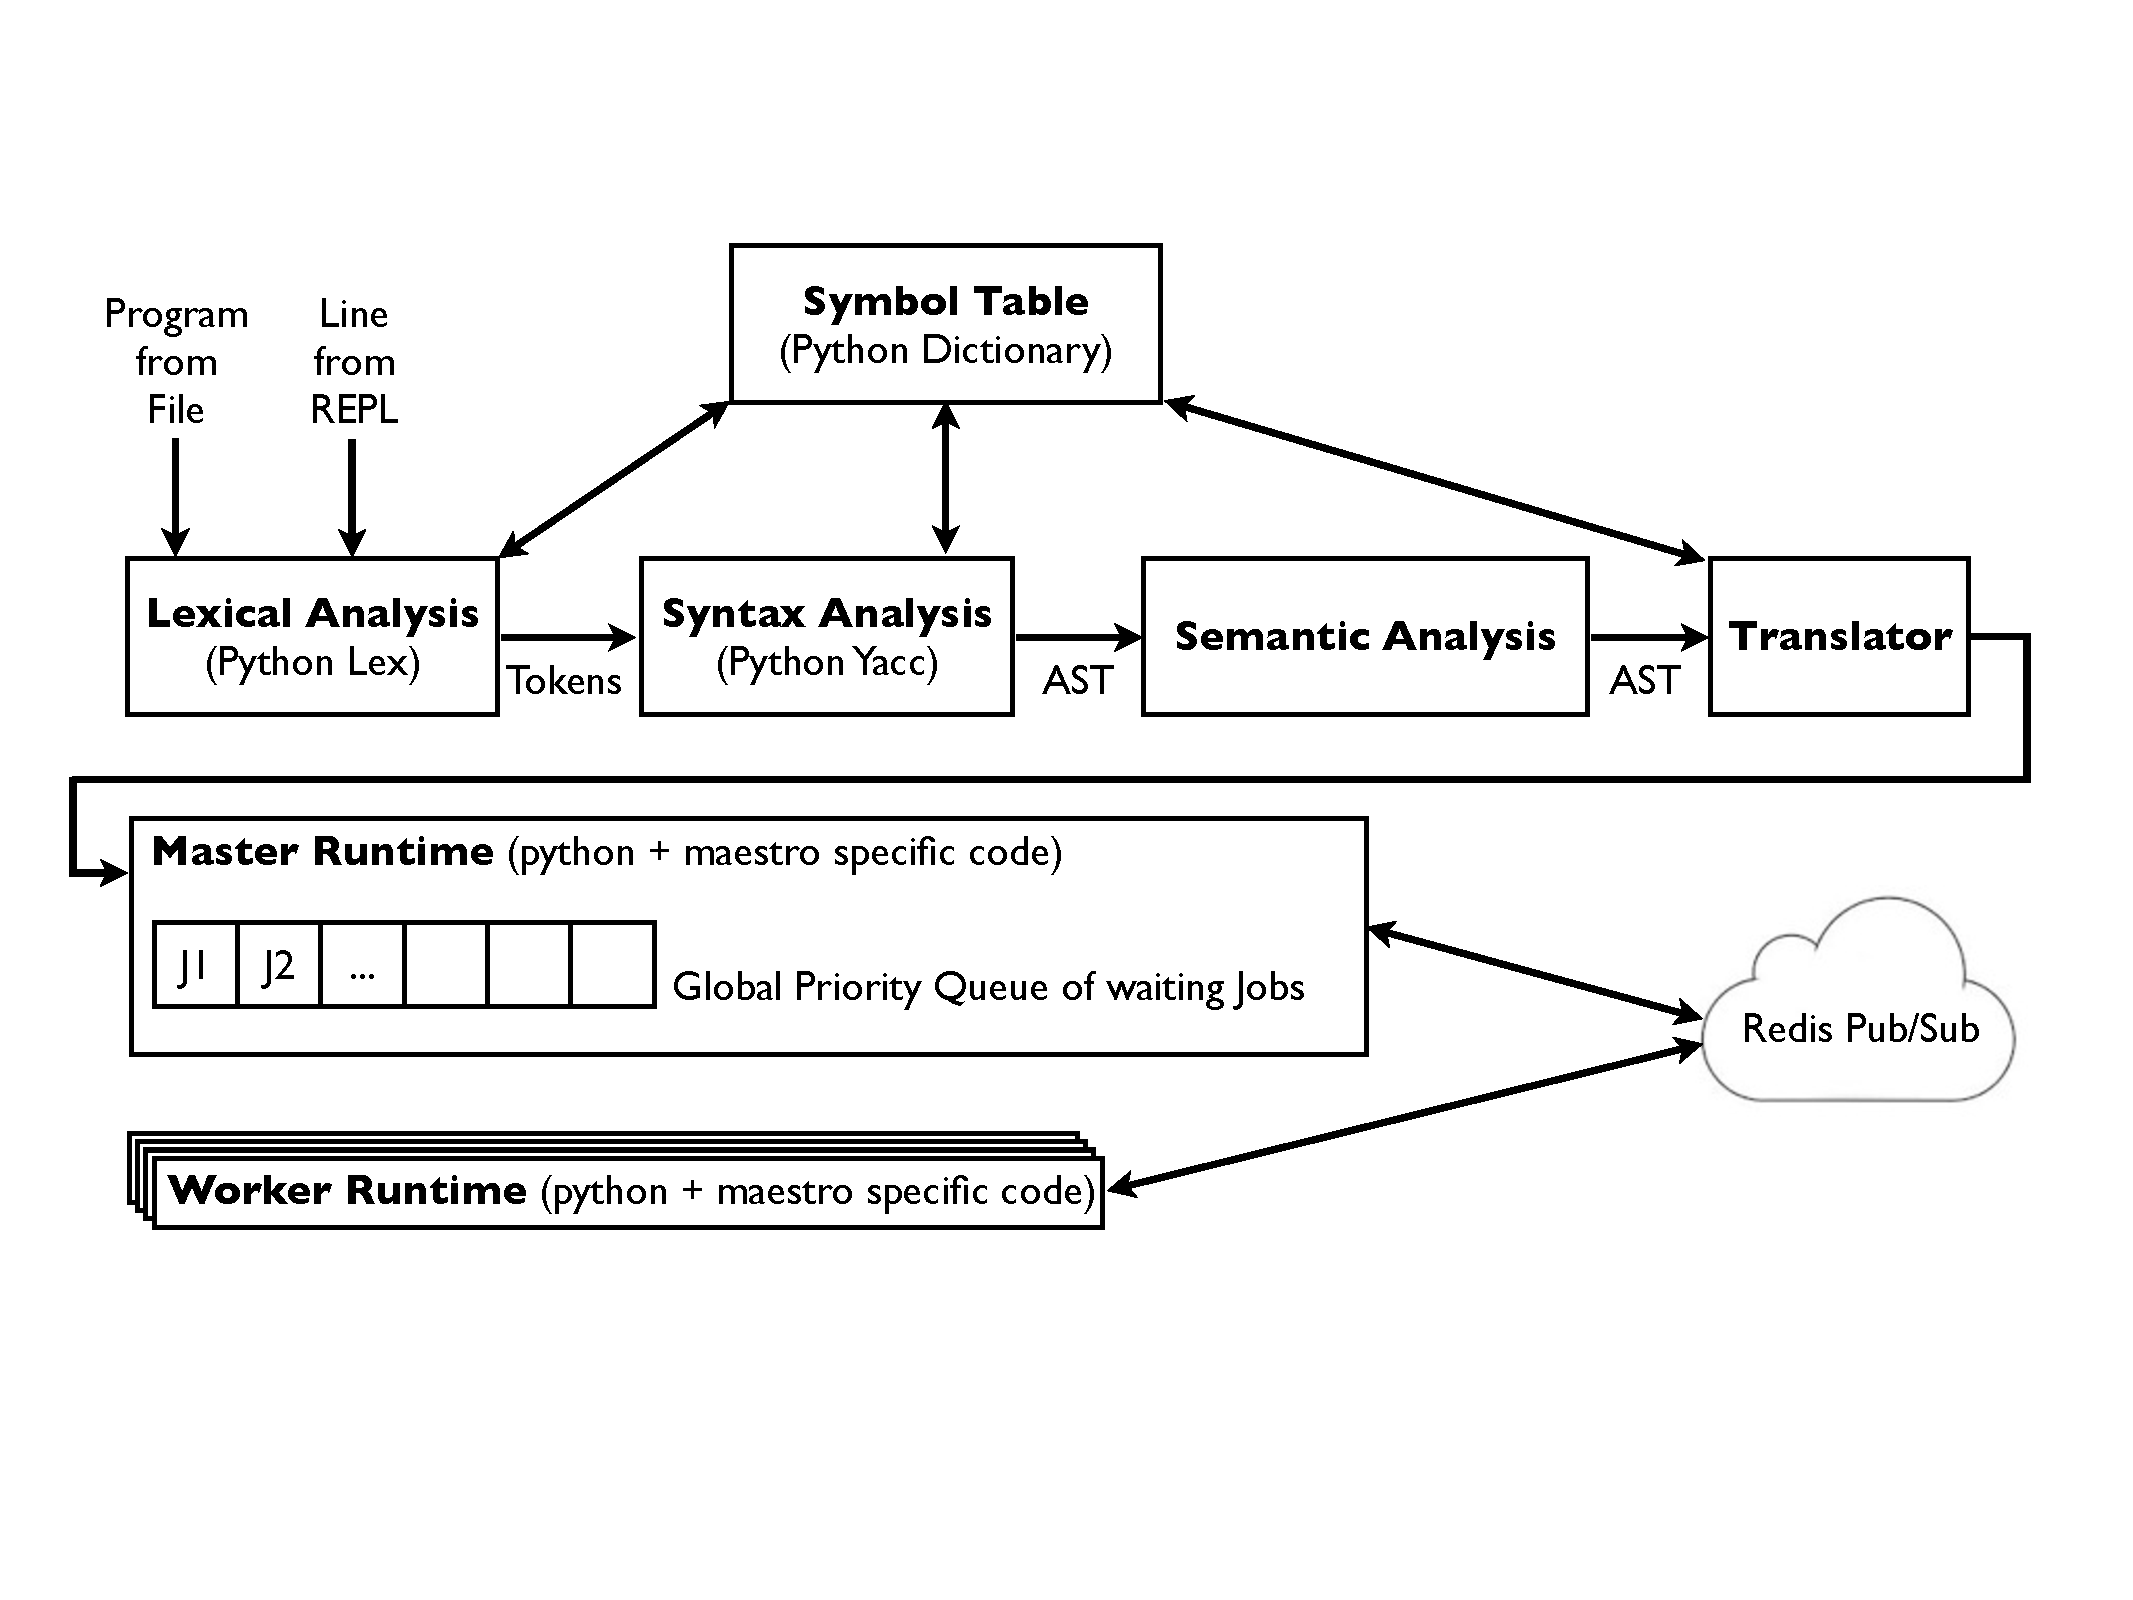
\includegraphics[width=15cm]{figures/archi.pdf}
  \caption{Maestro Architecture}
\label{fig:archi}
\end{figure}

\section{Interfaces}
The two main interfaces are the AST and the API. We will describe them in turn.

\paragraph{AST}

The AST is produced by the syntax analyser.
It is a tree with each node having children, or a value if it is itself a leaf.
The node also comprises the type of the expression it represents.
It is used by the syntax analyser and the translator.

\paragraph{API}

The API is exposed by the backend, and gives Maestro-specific features to the translator.
In particular, it exposes a Job object, central to our language, and functions to set dependencies and add Jobs
to the run queue.

\section{Modules}

\paragraph{Lexer}

The lexer takes the program or the REPL lines, and produces tokens for the syntax analyser.
Comments are discarded by the lexer directly.

The Lexer was written by Mathias with PLY.

\paragraph{Syntax Analyser}

The Syntax Analyser contains the grammar for Maestro, and uses the lexer's output to produce the AST using bottom-up parsing and an S-attribute SDD.

The Syntax Analyser was written with PLY. Mathias wrote the grammar and SDD and Georgios handled error recovery.

\paragraph{Semantic Analyzer}

The Semantic Analyser walks the AST to verify type compatibility and that variables were declared before being accessed.

The Semantic Analyser was written by Georgios.

\paragraph{Translator}

The translator translates the AST into Python and executes it.
It is coded as a recursive function that keeps track of computed values and types.
It makes extensive use of the backend API for Job creation and management, and leverages python expressiveness to implement complex features like map/reduce and dynamic code dependencies.

The translator was written by Mathias.

\paragraph{Backend}

The Backend exposes Maestro specific abstraction and handles the Job scheduling and distribution.
Because it's fairly complex and interesting,  but doesn't have its own section, we descibe it in more length here.
To support \lang{}'s job scheduling and dispatching for remote execution, we
built a distributed communication protocol whose main components are: (i)
a local job queue, (ii) a Redis
publish/subscribe communication channel, and (iii) a pool of workers dedicated
to job execution. The local job queue is used to keep track of active jobs
and their dependencies and is bound to a runtime environment. A custom Daemon
spins periodically on the job queue and dispatches for execution jobs with
resolved dependencies. Since job execution is either local or remote, job
dispatching is optional. On local execution, the job dispatcher requests a
shell on the local machine for job execution. On remote execution, the job
dispatcher sends requests to check which are the active workers on the Redis
channel, and afterwards dispatches (publishes) a job to the channel. One of the
subscribed active workers executes the job and sends back the output, on a job
specific redis channel. When the runtime Daemon receives the output of the
dispatched job via the job-specific channel, it prints its stdout and also
saves it in a log file under the current working directory.

Most of the Backend code was written by Vaggelis. Georgios and Mathias added some glue and small features.

\paragraph{Testing}:
Testing is a key part of any complex software system.
This is why it was assigned two persons.
Our testing framework will be described in details in a later chapter.

The testing frameworks and most of the tests were written by Arun and Yiren, and integrated from informal tests used by developers of new features.


\section{Organization}
The hard thing with a multi-person project with many parts depending on each other is figuring out a way to all work in parallel.
Even if we didn't always succeed, we took several steps to maximize parallelism.
First, we had an early "hello world" program working by implementing a basic lexer and semantic analyser and a basic backend.
We did not produced an AST and called backend functions directly, but having an end to end program helped a great deal in thinking about more advanced features we wanted.

We then added the production of an AST from the lexical analyser, while still computing values on the fly to keep being able to run programs.
This allowed us to add semantic analysis, and work on the translator that traverses the AST.
When we finally switched to working on a translator, adding features from the backend like remote Jobs was much easier.

\chapter{Development and Run-time Environment}
\section{sect:Development}
Our interpreter was developed under a Unix-based environment, specifically Debian, Ubuntu and MacOS.
Every member used their favorite text editor. Mainly vim and sublime. We used Github to host our
repository. As version control system we used Git. Also some of us used tig for terminal access git in
text mode. We did not used any issue tracking tool as 
our main development was done synchronous with all members being in the same room.
Our presentation was created, edited and distributed with Google Drive.


We used Python 2.7.3 and the Python-Lex-Yacc (PLY) to create and test our language. A generic Makefile
was created for the purpose of running all tests at once. Most of our examples are bash scripts.
For more sophisticated scripts such as map-reduce, we used ruby.


Our interpreter can take a file as argument. Also a REPL is started if no argument
is specified by the user.

\section{Runtime Environment}
One of our main goals of maestro is to distribute jobs and test them in computers with different
architecture, different operating systems and many more. Because of this our environment should have
a small number or even none environment dependencies. In favor of this our interpreter has 2 running options. 
At the end small changes are needed for the distributed functionality.
What our interpreter needs is a pc that can connect to the internet and the ability to spawn threads. 
Many packages from python are needed such as
\textit{ 
\item pip install redis
\item pip install colorama
}
Our user does not need to have a redis server running. A machine on the internet that has redis server
will be used as a master(channel). User only wants the ip of the machine and the port redis is listening.
Otherwise he can run it locally with no environment change.
\subsection{Local}
When run locally our interpreter is creating processes to run jobs.
No changes needed in the environment.
\subsection{Distributed}
For distributed run also needs a redis server for publishing messages with a master and a worker. 
Both of them can be also be done in localhost.
For creating a master user must specify \textit{service(IP:PORT)}. For worker he must
specify \textit{worker(IP:PORT)}. Both of these examples are handled by our interpreter.




 

\chapter{Test Plan}
\section{Methodology}
We do not rely on any existing Python unit-test framework for our testing purposes. Instead, we have developed a customized testing engine for our project. The engine, encapsulated by the Tests folder, comprises of several Python files. Each file consists of a test written in Maestro that checks both the robustness of the compiler (i.e. its ability to identify and parse tokens), and the final output of the program. 

Presented below is a sample unit test.

\begin{center}
\begin{verbatim}
#!maestro
master("0.0.0.0:6379");
# check what happens when a job is run without being declared
a = Job('print.py', 'foo');
c = Job('print.py' 'bar');
run(a -> b -> c);  # Job b is not declared
\end{verbatim}
\end{center}

The test first checks if two Jobs are created successfully. The file \textit{print.py} is a Python program that writes the argument passed to it to a file \textit{check.txt}. Once executed, Job \textit{a} must run the argument \textit{foo} through the program \textit{print.py}. Similarly, Job \textit{b} must run the argument \textit{bar} through \textit{print.py}. 
Once the two Jobs have been created successfully, we attempt to pass an undeclared Job to the \textit{run} method, which executes a single Job or a list of Jobs in the given order. In this case, we check to see if the Maestro compiler identifies undeclared Job \textit{b} as an error and handles it elegantly. Once the test completes execution, we check the expected output against the output that was piped to \textit{check.txt} to confirm success or failure. 

We have a total of 15 testcases in our engine that test Maestro's  overall performance in different steps.

\section{Relevant Files and Descriptions}

\textbf{testframework.py}
\newline
\indent This is the main framework file. It can execute all Maestro test-cases or individual ones, depending on how it is called. 
\newline \textit{python testframework.py all} executes all test cases in the \textit{Tests} folder. Replacing \textit{all} with the test-name will execute individual tests. 
\newline
\newline
\textbf{run.sh}
\newline
\indent Similar to testframework.py, but written in bash script.
\newline
\newline
\textbf{Tests\textbackslash print.py}
\newline
\indent This program is run by every Job created in our test cases. It writes the argument that it receives into file \textit{check.txt}. 
\newline
\newline
\textbf{Tests\textbackslash}
\newline
\indent This folder contains all 75 Maestro test cases.
\newpage
\noindent\textbf{TestsOutput\textbackslash check.txt}
\newline
\indent The checkfile to which \textit{print.py} writes its output. We compare the contents of the file against the expected output to determine success or failure of a given Job.
\newline
\newline

\section{Selected Test Cases}
\begin{enumerate}

\item This test checks the performance of Maestro in presence of a circular dependency. 
\begin{verbatim}
#!maestro

a = Job("./tmp/test.sh", "bla");
b = Job("./tmp/test.sh", "foo");
c = Job("./tmp/test.sh", "chk");

run(a->b->c->a); //there is a circular dependency here
\end{verbatim}
Here job \textit{a} depends on \textit{b}, \textit{b} depends on \textit{c} and job \textit{c} in-turn depends on job \textit{a}.

\item This test checks the performance of Maestro on self dependencies.

\begin{verbatim}
#!maestro

a = Job("./tmp/test.sh", "bla");
b= Job("./tmp/test.sh", "bla");

run(a->a); //self-dependency
\end{verbatim}

Here job \textit{a} depends on itself.
\newpage
\noindent \item This test checks Maestro's response to an instance of imbalanced parenthesis.

\begin{verbatim}
#!maestro

a = Job("./tmp/test.sh", "bla");
b= Job("./tmp/test.sh", "foo"; //Imbalanced parenthesis
c = Job("./tmp/test.sh", "bla");

run(a);
\end{verbatim}

\item This test case checks what happens when we provide a Map-Reduce job to maestro.

\begin{verbatim}
#! maestro

a = Job("./cut.rb", "./all.txt", "3");

maps = map(a, "./count.rb", 3);
red = reduce(maps, "./reduce.rb");

run(a, maps, red);
\end{verbatim}

\end{enumerate}


\chapter{Conclusions}

\section{Lessons learned as a team (to be written by the entire team)}
\begin{itemize}
\item For a large project such as this one, it is important to have a gameplan ready ahead of time. It was especially apparent to us that we needed to be able to manage our time well, since each team member gets exponentially busier as the semester matures. 
\item We learned to make full use of version control using GitHub. This helped each of us stay on track with others' progress, and stay in sync through the course of the semester.
\item Communication was key in making this project successful. We learned that we had to be able to talk to our team members with an open mind, and at the same time also make our point come across in a respectful way.
\end{itemize}


\section{Lessons learned by each team member (written by each team member)}
\begin{enumerate}
\item \textbf{Arun Swaminathan} \newline
Being a part of the team that built Maestro has been my first experience with working on a large-scale project. I learned a lot about how to work with a team and deliver code on time.
One of the biggest takeaways for me is my knowledge of the intrinsics of compilers. I had to dive into the nitty-gritty of what I, as a developer, had taken for granted for most of my coding lifetime. Being able to understand \textit{why} a compiler does what it does, \textit{how} it does it and understanding how all of its parts come together to make a robust piece of software is of the utmost importance.

\item \textbf{Yiren Lu} \newline
As much as modularity was emphasized in the instructions for the project, I
realized how difficult this is to implement in practice: chunking up the
compiler in such a way that every person can work independently (as opposed to
conditioned on someone else finishing their part) is practically an exercise in
gerrymandering. This was doubly hard in this instance, because the components
of a compiler come together more or less linearly - lexer, parser, ast,
semantic analysis. You can't do the semantic analysis without the AST; you
can't test nontrivial programs without the semantic analysis. Some of these
problems probably could have been avoided if we had a skeleton compiler working
front to back, early on in the semester - Mathias was actually very good about
putting the lexer and parser together before spring break - but some minor bugs
turned out to take longer than expected to fix. Something to remember for next
time.

\item \textbf{Vaggelis Atlidakis} \newline
Interaction and communication within a team of five member may seem trivial,
but it is not. The main challenge was that, although we all had
good programming skills, none of us had good knowledge of the procedure
involved in building a compiler. In order to contribute to the implementation
of \lang{}, we had to continuously learn new things and use them to contribute
to the evolution of our project. The biggest take-away from this join effort is
that good communication can drive great results.


\item \textbf{Mathias Lecuyer}
Knowing how a programming language works, with first hand experience, is very valuable.
I think it will help me to understand better about DSLs I use everyday, and ask the right questions about semantics when I create one (even if it's usually inside a language like Ruby than as a standalone language).
This is, I think, my main take away for this class. I also really enjoyed the more formal parts, especially lambda calculus.

My second take away is on the human side of programming, and especially parallelization.
This is not an easy to solve problem in software, and not surprisingly it is also tricky with developers.
Some people are not proactive in their involvement, and it is very easy to leave them aside.
However with the right push, they can make great contributions, and it is important to find the right job for them and integrate them.
What is hard but important is to avoid frustration between team members when some have a harder time to find a place in the project where they can bring value.
In our team, it seemed very linked to the separation of the project in well defined blocks.
We managed to split the project in only 3 well defined blocks on which we could work in parallel: frontend, backend, and testing.
This meant that it was hard for each of the five members to own a part of the code, and probably contributed to some lack of involvement in the project.
Moreover, testing was hard at the beginning because the language was breaking all the time and was not very well defined.
When we added the AST and the translation, we became more agile and the project was more stable, so it became easier to contribute.
I think that in the end every one of us could find a way to make very valuable contributions.


\item \textbf{Georgios Koloventzos}
Building an interpreter was quite a challenge. Using most of theory to go from an idea to a full-fledged interpreter
for distributing jobs. Understanding how lexer and parser really work in order to do dynamic type checking traversing
the abstrax syntax tree. Making decisions from how will structure the language to what will be the error message could change
how our language behaves. Simple decisions can restructure a lot what we have already implemented. Having done most of the work
in last week did not let us put all of our ideas to the language.
Nevertheless we have a strong distributed job orchestrator which maybe in future work to help scientist around the world
to test, execute and analyze tons of data.
\end{enumerate}
\section{Advice for future teams (written by the entire team)}
Two main pieces of advice that we would give to future teams: 1) Pick your language carefully and 2) Integrate continuously. When we were brainstorming project ideas, a couple of different ones were bandied around and we were very organized (probably the most organized ever) about listing their pros and cons. We were each assigned to do research and write sample programs for how we envisioned the language we came up with. Some other ideas that eventually weren't voted in were a probabilistic programming language as well as a language for creating recipes out of input food ingredients. After some discussion, we eventually picked Maestro.

We were lucky because Maestro turned out to be the right scope - it was organized around a central demand - being able to run jobs potentially in parallel or with dependences - so basically all aspects of the language bent to that imperative. It was also cleverly turing-complete. Since Maestro is a programming language to organize and run other programs, it can technically run any program that those programs can run.

The second piece of advice derives from something we did less well. It is tempting to say that we're done with 2/3 of the project when 2/3 of the pieces have been completed. But until all these pieces have been integrated, we've essentially done very little. Integration is the biggest challenge, and it gets harder the longer you wait to do it, not only because there are more pieces, but because it's harder to parallelize the work (other team members are more and more out of the loop). The optimal way to integrate is constantly. 
    
\section{Suggestions}
Each of us had different thoughts on which components of the class should be kept and tossed out, but here are a few that we were consistent on:

\begin{enumerate}
\item More referencing back and forth to the initial compiler diagram. Some of us often felt lost in the nitty gritty. For instance, it took until reviewing for the final exam to really realize the significance of Ershov numbers, and where they fit into the bigger picture.
\item Go more in depth in the first introduction to lambda calculus. Some of us had never taken the computer science theory course here (or had previously been exposed to lambda calculus but only superficially). For instance, beta reductions require that you replace all free instances of the variable in \emph{the expression}. But the variables that are free in the expression turn out to be bound in the abstraction. This was a source of confusion. 
\item If you're short on time, you can probably cut some of the arithmetic and boolean lambda calculus in the last lecture. There was too much to motivate properly, so many of us ended up trying to memorize the lambda abstractions for true and false, which undermines the spirit of lambda calculus in the first place.
\item We enjoyed the guest lectures. They were amusing and different and should be kept.
\end{enumerate} 

\chapter{Appendix}
\linespread{0.5}
\section{GIT Log}
\label{sect:appen}
\verbatiminput{./gitlog/sample_log.txt}

\section{Source Code}

\subsection{REPL (George)}
\verbatiminput{../src/run.py}
\verbatiminput{../src/maestro_cmd.py}

\subsection{Lexer (Mathias)}
\verbatiminput{../src/mlex.py}

\subsection{Parser (Mathias, George)}
\verbatiminput{../src/myacc.py}

\subsection{Test Framework (Arun, Yiren)}
\verbatiminput{../src/test_framework.py}

\subsection{Semantic Analysis (George)}
\verbatiminput{../src/pipeline/semantic_analysis.py}

\subsection{Semantic Actions (Mathias)}
\verbatiminput{../src/pipeline/translation.py}

\subsection{Backend (Vagelis, Mathias, and George)}
\verbatiminput{../src/helpers/jobs.py}
\verbatiminput{../src/helpers/workers.py}

\subsection{Job Dispatcher Daemon (Vaggelis)}
\verbatiminput{../src/helpers/jobqueue.py}



%\section{Source Code}
%...

\end{document}
